\section{The Information Flow}
\label{sec:architecture_flow}

Once the AdaptUI's layers and modules have been described, in this section the 
interaction among them and the information flow are reviewed.
Figure~\ref{fig:architecture_flow} shows a diagram with the whole architecture
and data flows.

First, and within the Modelling Layer, the user capabilities and context and
device characteristics are collected by the Capabilities Collector. This module
stores the collected information about these entities in Android using key-value
sets. While the capabilities of the device and several context parameters are
gathered transparently for the user, to collect his/her capabilities the
Capabilities Collector needs the user to complete a profile personalization process.

Once the Capabilities Collector finishes its task, the Semantic Modeller retrieves
the stored information and begins to transform it into semantics using the
AdaptUIOnt ontology. To be able to use semantics and to manipulate the model
and the available knowledge about the entities the Semantic Modeller uses
\textit{Pellet4Android}, which is an Android based port of Pellet.

Next, the Adaptation Engine (within the Adaptation Layer) semantically requests
the last adaptation instructions. These instructions are defined by the rules
triggered when the Semantic Modeller stores the knowledge in the AdaptUIOnt
ontology. Once it is stored, the corresponding rules result into a series of
adaptations. These adaptations, represented through the \textit{Adaptation}
class, are collected by the Adaptation Engine and represented in the user's display.

Once the user receives the corresponding adapted user interface, another Adaptation
Layer's module works in background: the Adaptation Polisher. Actually, this module
starts working from the beginning. Its purpose is to be aware of the user interaction
with the applications. This includes not only the adapted applications but also
the rest of them. Thus, it is able to establish several usability boundaries
under which the user might no be comfortable with. Comparing the user interaction
profile (generated during the usage of default applications under normal
circumstances) and the adapted interaction model (generated during the interaction
with an adapted user interface) this module triggers several instructions to
re-adapt the user interface. These instructions are ruled through the
post-adaptation set of rules.

Finally, within the Application Layer several tools (provided through an \ac{api})
are available for developers to make their applications adaptive and modify the
knowledge which will represent the domain (including concepts, relationships and
rules).

\begin{figure}
\centering
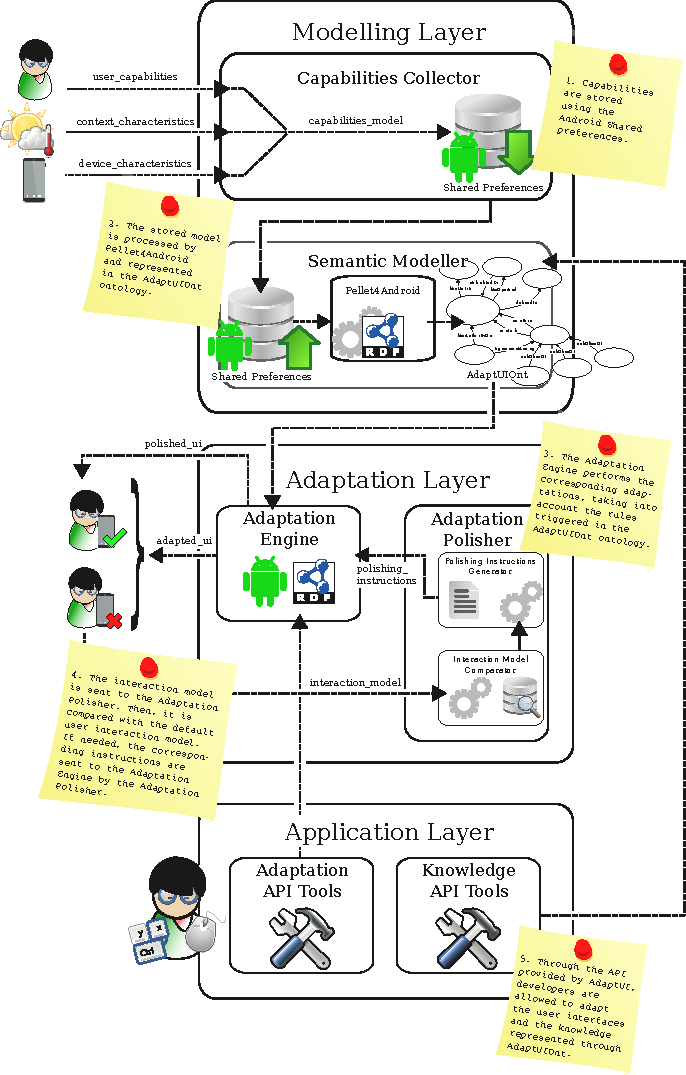
\includegraphics[width=0.85\textwidth]{architecture_flow.pdf}
\caption{The information flow within the AdaptUI platform.}
\label{fig:architecture_flow}
\end{figure}